\documentclass[usenatbib,usegraphicx,letterpaper]{mn2e}
\usepackage[totalwidth=480pt,totalheight=680pt]{geometry}

\usepackage{amssymb}
\usepackage{epsfig}
\usepackage{amsmath}
\usepackage{color}
\usepackage[dvipsnames]{xcolor}
%\usepackage{hyperref}
\usepackage{yfonts}
\usepackage{epsfig}  \usepackage{graphicx}   \usepackage{rotating}

\usepackage{listings, multicol}
\usepackage{caption}
\DeclareCaptionFont{white}{\color{white}}
\DeclareCaptionFormat{listing}{\colorbox{gray}{\parbox{\textwidth}{#1#2#3}}}
\captionsetup[lstlisting]{format=listing,labelfont=white,textfont=white}

%------- New commands

\newcommand{\lsim}{\lower0.6ex\vbox{\hbox{$ \buildrel{\textstyle <}\over{\sim}\ $}}}
\newcommand{\gsim}{\lower0.6ex\vbox{\hbox{$ \buildrel{\textstyle >}\over{\sim}\ $}}}
\newcommand{\beq}{\begin{equation}}
\newcommand{\eeq}{\end{equation}}

%------ Journals

\newcommand{\mnras}{Mon. Not. R. Astron. Soc.}
\newcommand{\apjl}{Astrophys. J. Lett.}
\newcommand{\aj}{Astron. J.}
\newcommand{\aap}{Astron. Astrophys.}
\newcommand{\araa}{Ann. Rev. Astron. Astroph.}
\newcommand{\apjs}{Astrophys. J. Suppl. Ser.}
\newcommand{\physrep}{Phys. Rep.}
\newcommand{\jcap}{JCAP}
\newcommand{\prd}{Phys. Rev. D}
\newcommand{\apj}{ApJ}

\newcommand{\wprp}{w_{\mathrm{p}}}
\newcommand{\rp}{r_{\mathrm{p}}}

\bibliographystyle{mn2e}


% misc 
\newcommand{\ben}{\begin{enumerate}}
\newcommand{\een}{\end{enumerate}}
\newcommand{\bit}{\begin{itemize}}
\newcommand{\eit}{\end{itemize}}

\newcommand{\rproj}{r_{\rm p}}

\newcommand{\mockobs}{{\tt mock\_observables }}
\newcommand{\emodels}{{\tt empirical\_models }}
\newcommand{\sims}{{\tt sim\_manager }}


\title[Presenting Halotools]
{
High-Precision Modeling of Large-Scale Structure: \\An open source approach with Halotools}

\author[Hearin et al.]
{Andrew P. Hearin$^{1}$, Duncan Campbell$^{2},$ Erik Tollerud$^{2,3}$\newauthor
many others \\
$^1$Yale Center for Astronomy \& Astrophysics, Yale University, New Haven, CT\\
$^2$Department of Astronomy, Yale University, P.O. Box 208101, New Haven, CT\\
$^3$Space Telescope Science Institute, Baltimore, MD 21218, USA}

\pagerange{\pageref{firstpage}--\pageref{lastpage}} \pubyear{}

\begin{document}

\maketitle
%----------------------------------------------------------------
%%%%%%%%%%%%%%%%%%%%%%%  A B S T R A C T %%%%%%%%%%%%%%%%%%%%%%%%%%%%%%

\begin{abstract}

We  present the first official release of Halotools (v0.2), a community-driven python package designed to build and test models of the galaxy-halo connection. Halotools provides a modular platform for creating mock universes with a rich variety of models of galaxy evolution, such as the HOD, CLF, abundance matching, assembly biased models, halo profiles, velocity bias, and many other model styles and features. The package has an extensive, heavily optimized toolkit to make mock observations on a synthetic galaxy population, including galaxy clustering, galaxy-galaxy lensing, galaxy group identification, RSD multipoles, void statistics, pairwise velocities and others. Halotools is written in a object-oriented style that enables complex models to be built from a set of simple, interchangeable components, including those of your own creation. Halotools has a rigorously maintained automated testing suite and is exhaustively documented on halotools.readthedocs.org, which includes quickstart guides, source code notes and a large collection of worked examples. The documentation effectively serves as an online textbook on how to build empirical models of galaxy formation with python. We conclude this paper by describing how Halotools can be used to constrain galaxy formation physics, and by outlining the Halotools program to help prepare for the arrival of Stage IV dark energy experiments.

\end{abstract} 

%---------------------------
\section{Introduction}
\label{section:introduction}
%---------------------------

Halotools is an affiliated package\footnote{\tt http://www.astropy.org/affiliated} of Astropy \citep{astropy}.

%---------------------------
\section{Package Overview}
\label{section:overview}
%---------------------------

Halotools is composed almost entirely in python with syntax that is compatible with both 2.7.x and 3.x versions of the language. Bounds-checking, exception-handling, and high-level control flow are always written in pure python. Whenever possible, performance-critical functions are written to be trivially parallelized using python's native {\tt multiprocessing} module. Halotools relies heavily on vectorized functions in {\tt Numpy} as a core optimization strategy. However, in many cases there is simply no memory efficient way to vectorize a calculation, and it becomes necessary to write explicit loops over large numbers of points. In such situations, care is taken to pinpoint the specific part of the calculation that is the bottleneck; that section, and that section only, is written in cython (or straight C as a last resort). 

Halotools is designed with a high degree of modularity, so that users can pick and choose the features that are suitable to their science applications. At the highest level, this modularity is reflected in the organization of the package into sub-packages. For Halotools v0.2, there are three major sub-packages. The \emodels sub-package described in \S\ref{subsection:empirical_models} contains the implementation of models of the galaxy-halo connection, as well as a flexible object-oriented platform for users to design their own models. The \mockobs sub-package described in \S\ref{subsection:mock_observables} contains a collection of functions that can be used to generate predictions for models in a manner that can be directly compared to astronomical observations. Many of the functions in \mockobs should also be of general use in the analysis of halo catalogs. The \sims sub-package described in \S\ref{subsection:sim_manager} is responsible for reducing ``raw" halo catalogs into efficiently organized fast-loading hdf5 files, and for creating and keeping track of a persistent memory of where the simulation data is stored on disk. 

Although these sub-packages are designed to work together, each individual sub-package has entirely stand-alone functionality that is intended to be useful even in the absence of the others. For example, while Halotools does not provide pre-processed halo catalogs from the Millennium simulation, the \sims sub-package can nonetheless be used to process and cache Millennium halos into a convenient, self-expressive format that users of that simulation may find useful. The \emodels sub-package can be used to populate mock galaxies into the the halos of any cosmological simulation, where the populated halos could be identified by any algorithm. The functions in the \mockobs sub-package simply accept point-data as inputs, and so these functions could be used to generate observational predictions for semi-analytical models that otherwise have no connection to Halotools. 

In the subsections below we outline each of these sub-packages in turn, though we refer the reader to {\tt halotools.readthedocs.io} for more comprehensive descriptions. 

%---------------------------
\subsection{Empirical Models}
\label{subsection:empirical_models}
%---------------------------

%---------------------------
\subsection{Mock Observations}
\label{subsection:mock_observables}
%---------------------------

%%%%%%%%%%%%%%%%%%%%%%%%% FIGURE %%%%%%%%%%%%%%%%%%%%%%%%%%%%%
\begin{figure*}
\begin{center}
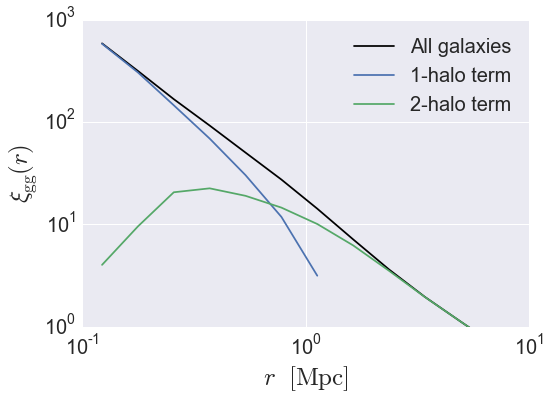
\includegraphics[width=8.3cm]{./FIGS/one_two_halo_clustering.png}
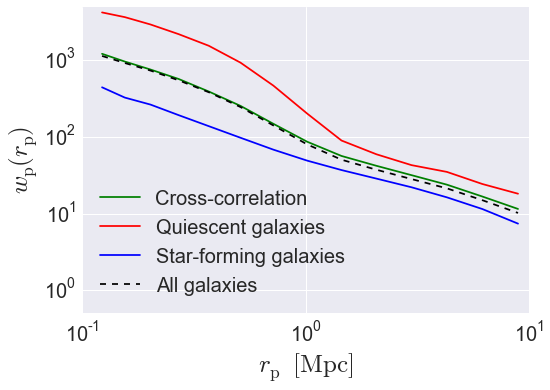
\includegraphics[width=8.3cm]{./FIGS/wp_red_blue_cross.png}
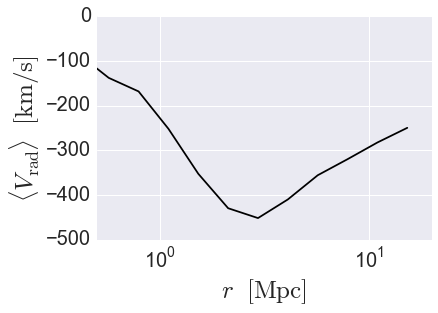
\includegraphics[width=8.3cm]{./FIGS/cluster_bcg_infall_velocity.png}
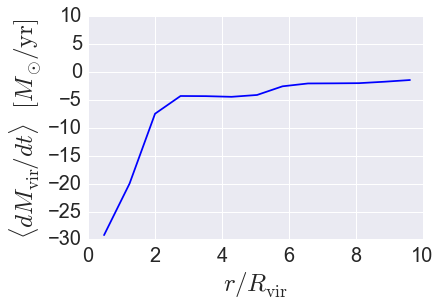
\includegraphics[width=8.3cm]{./FIGS/radial_profile_halocat_tutorial_fig1.png}
\caption{
Four example calculations done with Halotools demonstrating the diversity of the \mockobs sub-package. Each is part of a tutorial found in {\tt http://halotools.readthedocs.io}, to which we refer the reader for details. Here we only point out that each panel demonstrates the result of a heavily optimized function with a user-friendly API requiring minimal setup. {\em Top left:} Three-dimensional correlation function of mock galaxies $\xi_{\rm gg}(r)$ split into contributions from pairs of galaxies occupying a common halo (1-halo term), and pairs in distinct halos (2-halo term). {\em Top right:} Projected correlation function $w_{\rm p}(\rproj)$ of star-forming and quiescent galaxies, as well as their cross-correlation. {\em Bottom left:} Mean pairwise radial velocity of galaxies in the neighborhood of a cluster BCG. {\em Bottom right:} As a function of the $R_{\rm vir}-$normalized distance to a cluster, we show the mean mass accretion rate of nearby lower-mass subhalos. 
}
\label{fig:satcen}
\end{center}
\end{figure*}
%%%%%%%%%%%%%%%%%%%%%%%%%%%%%%%%%%%%%%%%%%%%%%%%%%%%%%%%%%%%%%%%%%%%

In the analysis of halo and (mock) galaxy catalogs, many of the same calculations are performed over and over again. How many pairs of points are separated by some distance $r$? What is the two-point correlation function of some sample of points? What is the host halo mass of some sample of subhalos? What is the local environmental density of some collection of galaxies? It is common to calculate the answers to these and other similar questions in an MCMC-type analysis, when high-performance is paramount. Even outside of the context of likelihood analyses, the sheer size of present-day cosmological simulations presents a formidable computational challenge to evaluate such functions in a reasonable runtime. There is also the notorious complicating nuisance of properly accounting for the periodic boundary conditions of a simulation. Much research time has been wasted by many different researchers writing their own private versions of these calculations, writing code that is not extensible as it was developed making hard assumptions that are only applicable to the immediate problem at hand. 

The {\tt mock\_observables} sub-package is designed to remedy this situation. This sub-package contains a large collection of functions that are commonly encountered when analyzing halo and galaxy catalogs, including:

\bit
\item The many variations of two-point correlation functions, 
\bit
\item three-dimensional correlation function $\xi(r),$ 
\item redshift-space correlation function $\xi(\rproj, \pi),$
\item projected correlation function $w_{\rm p}(\rproj),$
\item projected surface density $\Delta\Sigma(r_{\rm p})$ (aka galaxy-galaxy lensing),
\item RSD multipoles $\xi_{\ell}(s).$
\eit
\item marked correlation functions $\mathcal{M}(r),$
\item friends-of-friends group identification,
\item {\em group aggregation} calculations, e.g., calculating the total stellar mass of galaxies of a common group $M_{\ast}^{\rm tot},$
\item {\em isolation criteria}, e.g., identifying those galaxies without a more massive companion inside some search radius, 
\item pairwise velocity statistics, e.g, the line-of-sight velocity dispersion as a function of projected distance $\sigma_{\rm los}(\rproj),$
\item void probability function $P_{\rm void}(r).$
\eit

The \mockobs sub-package contains heavily optimized implementations of all the above functions, as well as a variety of others. Every function in \mockobs has a stable, user-friendly API that is consistently applied across the package. The docstring of all functions contains an explicit example of how to call the function, and in many cases there is a step-by-step tutorial showing how the function might be used in a typical analysis. Considerable effort has been taken to write \mockobs to be modular, so that users can easily borrow the algorithm patterns to write their own variation on the provided calculations. 

%---------------------------
\subsection{Managing Simulation Data}
\label{subsection:sim_manager}
%---------------------------

One of the most tedious tasks in simulation analysis is the initial process of getting started with a halo catalog: reading large data files storing the halos (typically ASCII-formatted), making cuts on halos, adding additional columns, and storing the reduced and value-added catalog on disk for later use. In our experience with simulation analysis, one of the most common sources of bugs comes from these initial bookkeeping exercises. 

The \sims sub-package has been written to standardize this process so that users can get started with full-fledge halo catalog analysis from just a few lines of code. The {\tt sim\_manager.RockstarHlistReader} class allows users to quickly create a Halotools-formatted catalog starting from the typical ASCII output of the {\tt Rockstar} halo-finder \citep{rockstar_trees, behroozi_rockstar11}. Users wishing to work with catalogs of halos identified by algorithms other than {\tt Rockstar} can use the {\tt sim\_manager.TabularAsciiReader} class to initially process their ascii data. Both readers are built around a convenient API that uses Python's native ``lazy evaluation" functionality to select on-the-fly only those columns and rows that are of interest, making these readers highly memory efficient. 

All Halotools-formatted catalogs are python objects storing the halo catalog itself in the form of an Astropy Table, and also storing some metadata about the simulated halos. In order to build an instance of a Halotools-formatted catalog, a large collection of self-consistency checks about the halo data and metadata are performed, and an exception is raised if any inconsistency is detected. These checks are automatically carried out at the initial processing stage, and also every time the catalog is loaded into memory, to help ensure that the catalog is processed correctly and does not become corrupt over time. 

The \sims sub-package allows users to cache their processed halo catalogs when they are saved to disk, creating the option to load their catalogs into memory with simple and intuitive syntax: 

\begin{lstlisting}[float=*t, label=some-code,caption = Loading a cached halo catalog into memory]
from halotools.mock_observables import CachedHaloCatalog
halocat = CachedHaloCatalog(simname = `bolshoi', redshift = 0.5)

print(halocat.halo_table[0:9]) # view the first few halos in the catalog
print(halocat.Lbox, halocat.particle_mass) # check halo catalog metadata
\end{lstlisting}

The cached simulations are stored in the form of an hdf5 file.\footnote{\tt http://www.h5py.org}. This binary file format is fast-loading and permits metadata to be bound directly to the file in a transparent manner, so that the cached binary file is a self-expressive object. The {\tt sim\_manager.HaloTableCache} class provides an object-oriented interface for managing the cache of simulations, but users are also free to work directly with the cache log, which is a simple, human-readable text file stored in \$HOME/.astropy/cache/halotools/halo\_table\_cache\_log.txt.

Using the Halotools caching system is optional in every respect. Users who prefer their own system for managing simulated data are free to do so in whatever manner they wish; they need only pass the necessary halo data and metadata to the {\tt sim\_manager.UserSuppliedHaloCatalog} class, and the full functionality of all sub-packages of Halotools works with the resulting object instance.  

The Halotools developers manage a collection of pre-processed halo catalogs that are available for download either with the {\tt sim\_manager.DownloadManager} class, or with the command-line script {\tt halotools/scripts/download\_additional\_halocat.py}. Through either download method, the catalogs are automatically cached and science-ready as soon as the download completes. Halotools currently offers pre-processed halo catalogs for Rockstar-identified halos from four different simulations: {\tt bolshoi, bolshoi-planck, consuelo} and {\tt multidark}, for which snapshots at $z=0, 0.5, 1$ and $2$ are available.


%---------------------------
\section{Package Development}
\label{section:development}
%---------------------------

\subsection{GitHub workflow}
\label{subsection:githubworkflow}

Halotools has been developed fully in the open since the inception of the project. Version control for the code base is managed using git\footnote{\tt http://git-scm.com}, and the public version of the code is hosted on GitHub\footnote{\tt http://www.github.com}. The latest stable version of the code can be installed via {\tt pip install halotools}, but at any given time the {\tt master} branch of the code on {\tt https://github.com/astropy/halotools} may have features and performance enhancements that are being prepared for the next release. A concerted effort is made to ensure that only thoroughly tested and documented code appears in the public {\tt master} branch, though Halotools users should be aware of the distinction between the bleeding edge version in {\tt master} and the official release version available through {\tt pip}. 

Development of the code is managed with a {\em Fork \& Pull} workflow. Briefly, code development begins by creating a private {\em fork} of the main repository on GitHub. Developers then work only on the code in their fork. In order to incorporate a change to the main repository, it is necessary to issue a {\em Pull Request} to the {\tt master} branch. The version of the code in the Pull Request is then reviewed by the Halotools developers before it is either rejected or merged into {\tt master}.

\subsection{Automated testing}
\label{subsection:testing}

Halotools includes hundreds of unit-tests that are incorporated into the package via the {\tt py.test} framework.\footnote{\tt http://pytest.org} These tests are typically small blocks of code that test a specific feature of a specific function. The purpose of the testing framework is both to verify scientific correctness and also to enforce that the API of the package remains stable. We also use {\em continuous integration}, a term referred to the automated process of running the entire test suite in a variety of different system configurations (e.g., with different releases of {\tt Numpy} and {\tt Astropy} installed, or different versions of the Python language). Each time any Pull Request is submitted to the {\tt master} branch of the code,the proposed new version of the code is copied to a variety of virtual environments, and the entire test suite is run repeatedly in each environment configuration. The Pull Request will not be merged into {\tt master} unless the entire test suite passes in all environment configurations. We use {\tt Travis}\footnote{\tt https://travis-ci.org} for continuous integration in Unix environments such as Linux and Mac OS X and {\tt AppVeyor}\footnote{\tt https://www.appveyor.com} for Windows environments. 

Pull Requests to the {\tt master} branch are additionally subject to a requirement enforced by {\tt Coveralls}.\footnote{\tt https://coveralls.io} This service performs a static analysis on the Halotools code base and determines the portions of the code that are covered by the test suite, making it straightforward to identify logical branches whose behavior remains to be tested. {\tt Coveralls} issues a report for the fraction of the code base that is covered by the test suite; if the returned value of this fraction is smaller than the coverage fraction of the current version of {\tt master}, the Pull Request is not accepted. This ensures that test coverage can only improve as the code evolves and new features are added. 

Any time a bug is found in the code, either by Halotools developers or users, a GitHub Issue is raised calling public attention to the problem. When the Halotools developers have resolved the problem, a corresponding {\em regression test} becomes a permanent contribution to the code base. The regression test explicitly demonstrates the specific source of the problem, and contains a hyperlink to the corresponding GitHub Issue. The test will fail when executed from the version of the code that had the problem, and will pass in the version with the fix. Regression testing helps makes it transparent how the bug was resolved and protects against the same bug from creeping back into the repository as the code evolves. 

\subsection{Documentation}
\label{subsection:documentation}

Documentation of the code base is generated via sphinx\footnote{\tt http://www.sphinx-doc.org} and is hosted on ReadTheDocs\footnote{\tt https://readthedocs.io} at {\tt http://halotools.readthedocs.io}. The public repository {\tt https://github.com/astropy/halotools} has a webhook set up so that whenever there is a change to the {\tt master} branch, the documentation is automatically rebuilt to reflect the most up-to-date version of {\tt master}. 

Every user-facing class, method and function in Halotools has a docstring describing its general purpose, its inputs and output, and also providing an explicit example usage. The docstring for many functions with complex behavior comes with a hyperlink to a separate section of the documentation in which mathematical derivations and algorithm notes are provided. The documentation also includes a large number of step-by-step tutorials and example analyses. The goal of these tutorials is more than simple code demonstration: the tutorials are intended to be a pedagogical tool illustrating how to analyze simulations and study models of the galaxy-halo connection in an efficient and reproducible manner. 


%---------------------------
\section{Planned Features}
\label{section:planned_features}
%---------------------------

%%%%%%%%%%%%%%%%%%%%%%%%%%%%%% ACKNOWLEDGEMENTS %%%%%%%%%%%%%%%%%%%%%

\section{acknowledgments}


\bibliography{./halotools}









%------------------------------------------------
\end{document}
%------------------------------------------------
